\message{ !name(solution_hw2.tex)}\documentclass[12pt]{amsart}
\usepackage[margin=1.1in]{geometry}
\usepackage{graphicx}
\linespread{1.0}
\newcommand{\ZZ}{\mathbb{Z}}
\newcommand{\QQ}{\mathbb{Q}}
\newcommand{\RR}{\mathbb{R}}
\newcommand{\CC}{\mathbb{C}}
\newcommand{\HH}{\mathbb{H}}
\newcommand{\FF}{\mathbb{F}}

\newcommand{\rank}{\mathop\mathrm{rank}}
\newcommand{\supp}{\mathop\mathrm{supp}}
\newcommand{\tr}{\mathop\mathrm{tr}}
\newcommand{\Span}{\mathop\mathrm{span}}

\newcommand{\cl}[1]{\overline{#1}}
\newcommand{\Id}{\mathop\mathrm{Id}}
\newcommand{\Int}{\mathop\mathrm{int}}

\newcommand{\Exercise}[1]{\ \par\noindent\textbf{\em{[#1]}}\\}
\newcommand{\Subexe}[1]{\ \par\noindent\textbf{\em{(#1).}}~}
\newcommand{\Subsubexe}[1]{\ \par\indent\emph{(#1).}~}

\makeatletter
\renewcommand{\section}{\@startsection{section}{1}{0mm}
{-\baselineskip}{0.5\baselineskip}{\bf\leftline}}
\makeatother

\begin{document}

\message{ !name(solution_hw2.tex) !offset(-3) }

\noindent CSci 5512 -- Artificial Intelligence II \hfill Jiecao Chen \hfill ID:4716311 \\
\textsc{Homework \#1 \hfill Due: Due Wed, Feb 20}\\

\section*{Question 1} 
\subsection*{a}
$P(C|r,w,s)\\
\indent =\alpha P(C,r,w,s)\\ 
\indent =\alpha P(C)P(r|C)P(s|C)P(w|s,r)\\
\indent =\alpha \langle 0.5,0.5\rangle\langle 0.8,0.2\rangle\langle 0.1,0.5\rangle\times 0.99\\
\indent =\alpha \langle 0.0396,0.0459\rangle\\
\indent =\langle 0.4444,0.5556\rangle$\\

$P(C|\neg r,w,s)\\
\indent =\alpha P(C,\neg r,w,s)\\ 
\indent =\alpha P(C)P(\neg r|C)P(s|C)P(w|s,\neg r)\\
\indent =\alpha \langle 0.5,0.5\rangle\langle 0.2,0.8\rangle\langle 0.1,0.5\rangle\times 0.90\\
\indent =\alpha \langle 0.009,0.18\rangle\\
\indent =\langle 0.047619,0.952381\rangle$\\


$P(R|c,w,s)\\
\indent =\alpha P(c,R,w,s)\\ 
\indent =\alpha P(c)P(R|c)P(s|c)P(w|s,R)\\
\indent =\alpha 0.5\times \langle 0.8,0.2\rangle\times 0.1 \times \langle 0.99,0.90\rangle\\
\indent =\alpha \langle 0.0396, 0.009\rangle\\
\indent =\langle 0.814815, 0.185185\rangle$\\

$P(R|\neg c,w,s)\\
\indent =\alpha P(\neg c,R,w,s)\\ 
\indent =\alpha P(\neg c)P(R|\neg c)P(s|\neg c)P(w|s,R)\\
\indent =\alpha 0.5\times \langle 0.2,0.8\rangle\times 0.5 \times \langle 0.99,0.90\rangle\\
\indent =\alpha \langle 0.0495, 0.18\rangle\\
\indent =\langle 0.215686, 0.784314\rangle$\\
PS: The first part is assigned as True and the second \textbf{False}

% \section*{Question 2} 
% \begin{figure}[h]
%   \centering
%   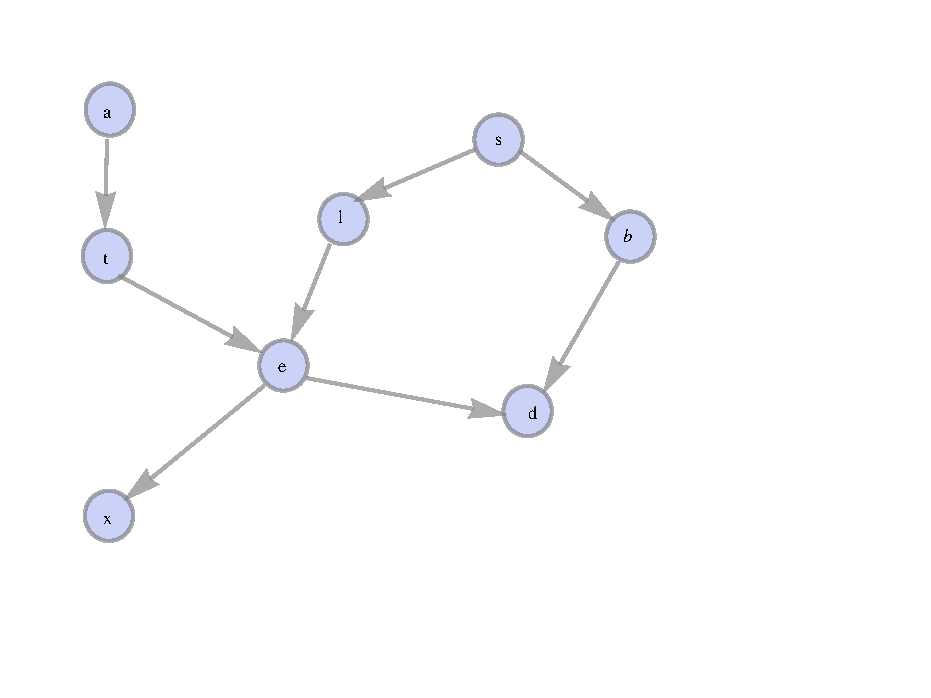
\includegraphics[width=0.8\textwidth]{fig2.pdf}
%   \caption{The Chest Clinic network}
% \end{figure}

% \subsection*{a}
% State if the following conditional independence are true or false:
% \subsubsection*{i} $t\bot s|d$\\
% Use D-separation or D-connection. 
% In the undirected path $t-e-d-b-s-b-s$, $d$ is a collider, thus $t$ and $s$ are D-connected, thus $t\bot s|d$ is false.
% \subsubsection*{ii} $l\bot b|s$\\
% $s$ is not a collider, thus $t\bot s|d$ is true.
% \subsubsection*{iii} $a\bot s|l,d$\\
% There are only two undirected paths from $a$ to $s$, one is  $a-t-e-d-b-s$, all colliders in this path (i.e. $l$) is in $\{l,d\}$, and all non-colliders are not in $\{l,d\}$, thus $a\bot s|l,d$ is false.

% \subsection*{b}
% We use bold font to stand fixed variables, thus
% $P(\mathbf{s}|\mathbf{a},\mathbf{x,b})=\frac{P(\mathbf{s,a,x,b})}{P(\mathbf{a,x,b})}$\\
% $P(\mathbf{s,a,x,b})
% =\sum_{e,t,l}P(\mathbf{s})P(\mathbf{a})P(\mathbf{b|s})P(\mathbf{x}|e)P(e|t,l)P(t|\mathbf{a})P(l|\mathbf{s})
% \\ \indent \indent =P(\mathbf{s})P(\mathbf{a})P(\mathbf{b|s})\sum_{t}P(t|\mathbf{a})
% \sum_{l}P(l|\mathbf{s})
% \sum_{e}P(\mathbf{x}|e)P(e|t,l)$\\
% \\
% $P(\mathbf{a,x,b})
% =\sum_{s,e,t,l}P(\mathbf{a})P(\mathbf{b}|s)P(s)P(\mathbf{x}|e)P(e|t,l)P(t|\mathbf{a})
% \\ \indent \indent =P(\mathbf{a})
% \sum_{s}P(\mathbf{b}|s)P(s)
% \sum_{l}P(l|s)
% \sum_{t}P(t|\mathbf{a})
% \sum_{e}P(\mathbf{x}|e)P(e|t,l)
% $
% \subsection*{c}
% If will know the value of $e$, then the computation complexity would significantly decrease. See the following formulas:\\
% $P(\mathbf{s}|\mathbf{a},\mathbf{x,b,e})=\frac{P(\mathbf{s,a,x,b,e})}{P(\mathbf{a,x,b,e})}$\\
% \\
% $P(\mathbf{s,a,x,b})
% =\sum_{e,t,l}P(\mathbf{s})P(\mathbf{a})P(\mathbf{b|s})P(\mathbf{x}|e)P(e|t,l)P(t|\mathbf{a})P(l|\mathbf{s})
% \\ \indent \indent =P(\mathbf{s})P(\mathbf{a})P(\mathbf{b|s})P(\mathbf{x}|\mathbf{e})
% \sum_{t}P(t|\mathbf{a})
% \sum_{l}P(l|\mathbf{s})
% P(\mathbf{e}|t,l)$\\
% \\
% $P(\mathbf{a,x,b})
% =\sum_{s,e,t,l}P(\mathbf{a})P(\mathbf{b}|s)P(s)P(\mathbf{x}|e)P(e|t,l)P(t|\mathbf{a})
% \\ \indent \indent =P(\mathbf{a})P(\mathbf{x|e})
% \sum_{s}P(\mathbf{b}|s)P(s)
% \sum_{l}P(l|s)
% \sum_{t}P(t|\mathbf{a})
% P(\mathbf{e}|t,l)
% $\\
% We no longer need to sum for the variable $e$.

% \section*{Question 3}
% \subsection*{(a)}
% See the Figure 2
% \begin{figure}[h]
%   \centering
%   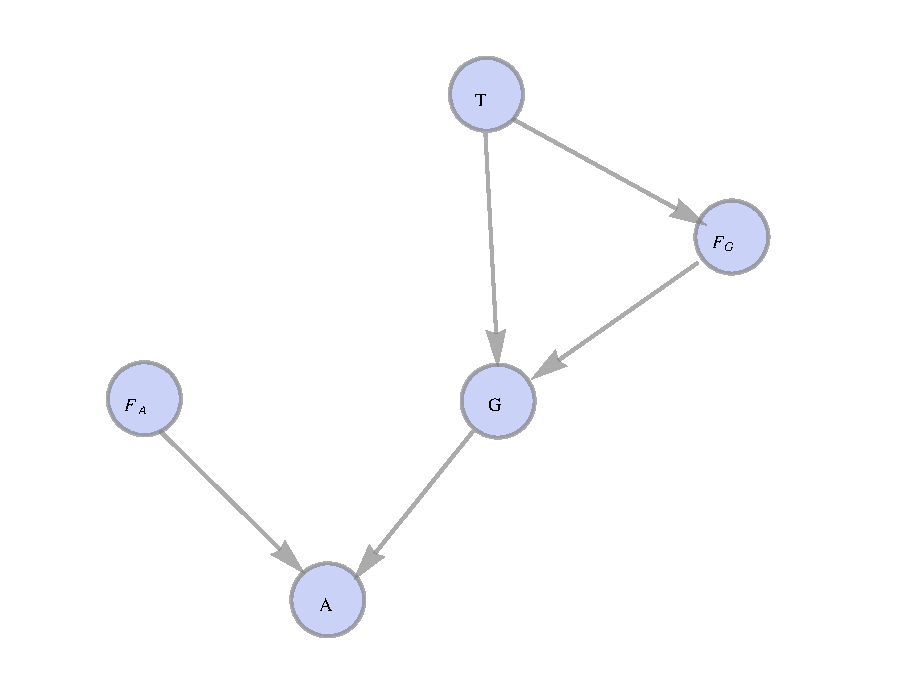
\includegraphics[width=0.7\textwidth]{temp.pdf}
%   \caption{Nuclear Temperature System Network}
% \end{figure}


% \subsection*{(b)}
% See Table 1.
% \begin{table}[h]
% \centering
% \caption{conditional prob table}
%     \begin{tabular}{| c c | c |}
%       \hline
%       $T$  & $F_G$  & $P(G=high|T,F_G)$ \\ \hline
%       high & faulty & $y$\\
%       high & work   & $x$\\
%       normal & faulty & $1-y$\\
%       normal & work   & $1-x$\\
%         \hline
%       \end{tabular}
% \end{table}


% \subsection*{(c)}
% See Table 2.
% \begin{table}[h]
% \centering
% \caption{conditional prob table}
%     \begin{tabular}{| c c | c |}
%       \hline
%       $G$  & $F_A$  & $P(A=sound|G,F_A)$ \\ \hline
%       high & faulty & $0$\\
%       high & work   & $1$\\
%       normal & faulty & $0$\\
%       normal & work   & $0$\\
%         \hline
%       \end{tabular}
% \end{table}

% \subsection*{(d)}
% we have notations: h-high, w-work, s-sound.\\
% $P(T=h|F_A=w,F_G=w,A=s)=\frac{P(T=h,F_A=w,F_G=w,A=s)}{P(F_A=w,F_G=w,A=s)}$, where\\
% $P(T=h,F_A=w,F_G=w,A=s)\\
% \indent \indent = P(T=h)P(F_A=w)P(F_G=w|T=h)\\
% \indent \indent \sum_{G}P(A=s|F_A=w,G)P(G|T=h,F_G=w)$\\
% $P(F_A=w,F_G=w,A=s)\\
% \indent \indent = P(F_A=w)\sum_{T}P(F_G=w|T)P(T)\sum_{G}P(A=s|F_A=w,G)P(G|T,F_G=w)$\\



% \section*{Question 4}
% \subsection*{(a)}
% \begin{figure}[h]
%   \centering
%   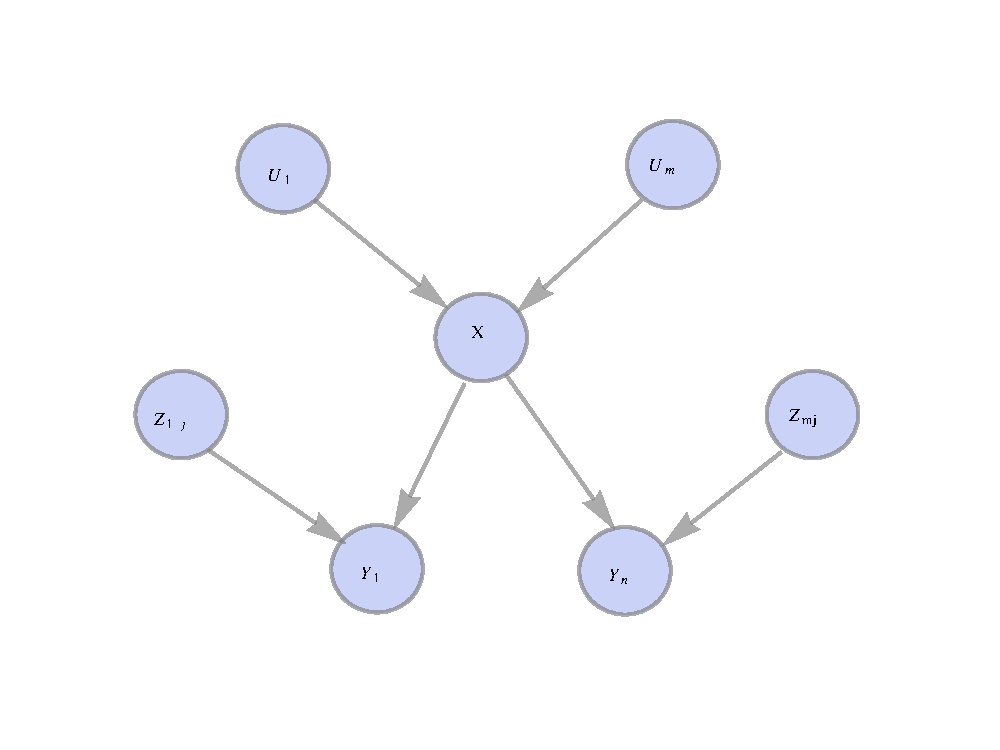
\includegraphics[width=0.7\textwidth]{pic.pdf}
%   \caption{Counterexample}
% \end{figure}

% We prove $P(X|\{U_i\},\{Z_j\})=P(X|\{U_i\})$ by contradiction:\\
% Assume $X$ and $\{Z_i\}$ are D-connected by $\{U_i\}$, then there exist $Z\in\{Z_i\}$
% such that there is a undirected path $U$ from $Z$ to $X$, and all its colliders are in $\{U_i\}$.\\
% \begin{enumerate}
% \item[{\textbf{case 1}}] $U\bigcap \{U_i\}=A\neq\emptyset$\\
% Since every node in $A$ is also in $\{U_i\}$, thus they are all non-colliders, in this case, 
% $X$ and $\{Z_i\}$ are D-connected by the path $U$.

% \item[{\textbf{case 2}}] $U\bigcap \{U_i\}=\emptyset$\\
% Thus $U\bigcap \{Y_i\}=A\neq\emptyset$, from the graph, if there is no collider in $A$, then 
% all arrows in $U$ are in the same direction (either from $Z\leftarrow X$ or $X\leftarrow Z$), but that's not true based on the graph in the question. So, there is at least one collider in $U$, but it is not in $\{U_i\}$, which contradicts to the assumption \textbf{“there exist $Z\in\{Z_i\}$
% such that there is a undirected path $U$ from $Z$ to $X$, and all its colliders are in $\{U_i\}$.”}
% \end{enumerate}
% We therefore have proved that $P(X|\{U_i\},\{Z_j\})=P(X|\{U_i\})$
% \subsection*{(b)}
% $P(X|\{U_i\},\{Y_j\},\{Z_j\})=P(X|\{U_i\},\{Y_j\})$ is no longer true, consider the following
% counterexample (see Figure 3):
% % insert graph
% \begin{figure}[h]
%   \centering
%   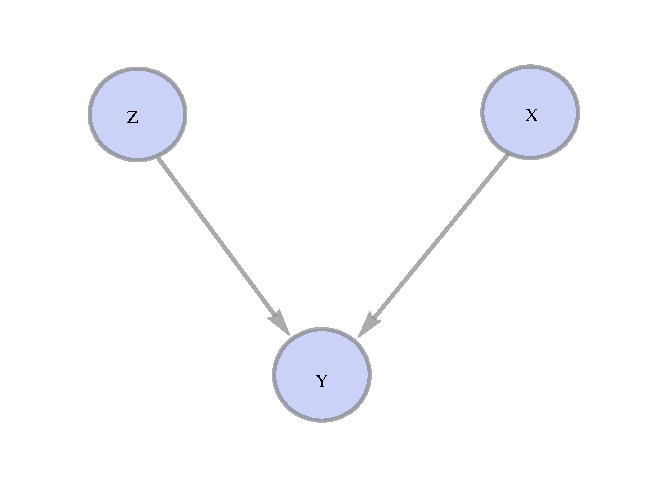
\includegraphics[width=0.5\textwidth]{ct_example.pdf}
%   \caption{Counterexample}
% \end{figure}

% In this case, $\{U_j\}=\emptyset$,$Y$ is a collider, thus $Z$ and $X$ are not conditional independent given $Y$.


\end{document} 




\message{ !name(solution_hw2.tex) !offset(-218) }
